\documentclass[12pt]{article}
\usepackage[left=1cm, right=1cm, top=2cm,bottom=1.5cm]{geometry} 

\usepackage[parfill]{parskip}
\usepackage[utf8]{inputenc}
\usepackage[T2A]{fontenc}
\usepackage[russian]{babel}
\usepackage{enumitem}
\usepackage[normalem]{ulem}
\usepackage{amsfonts, amsmath, amsthm, amssymb, mathtools,xcolor}
\usepackage{blkarray}

\usepackage{tabularx}
\usepackage{hhline}

\usepackage{accents}
\usepackage{fancyhdr}
\pagestyle{fancy}
\renewcommand{\headrulewidth}{1.5pt}
\renewcommand{\footrulewidth}{1pt}

\usepackage{graphicx}
\usepackage[figurename=Рис.]{caption}
\usepackage{subcaption}
\usepackage{float}

%%Наименование папки откуда забирать изображения
\graphicspath{ {./images/} }

%%Изменение формата для ввода доказательства
\renewcommand{\proofname}{$\square$  \nopunct}
\renewcommand\qedsymbol{$\blacksquare$}

%%Изменение отступа на таблицах
\addto\captionsrussian{%
	\renewcommand{\proofname}{$\square$ \nopunct}%
}
%% Римские цифры
\newcommand{\RN}[1]{%
	\textup{\uppercase\expandafter{\romannumeral#1}}%
}

%% Для удобства записи
\newcommand{\MR}{\mathbb{R}}
\newcommand{\MC}{\mathbb{C}}
\newcommand{\MQ}{\mathbb{Q}}
\newcommand{\MN}{\mathbb{N}}
\newcommand{\MZ}{\mathbb{Z}}
\newcommand{\MTB}{\mathbb{T}}
\newcommand{\MTI}{\mathbb{I}}
\newcommand{\MI}{\mathrm{I}}
\newcommand{\MCI}{\mathcal{I}}
\newcommand{\MJ}{\mathrm{J}}
\newcommand{\MH}{\mathrm{H}}
\newcommand{\MT}{\mathrm{T}}
\newcommand{\MU}{\mathcal{U}}
\newcommand{\MV}{\mathcal{V}}
\newcommand{\MB}{\mathcal{B}}
\newcommand{\MF}{\mathcal{F}}
\newcommand{\MW}{\mathcal{W}}
\newcommand{\ML}{\mathcal{L}}
\newcommand{\MP}{\mathcal{P}}
\newcommand{\VN}{\varnothing}
\newcommand{\VE}{\varepsilon}
\newcommand{\dx}{\, dx}
\newcommand{\dy}{\, dy}
\newcommand{\dz}{\, dz}
\newcommand{\dd}{\, d}


\theoremstyle{definition}
\newtheorem{defn}{Опр:}
\newtheorem{rem}{Rm:}
\newtheorem{prop}{Утв.}
\newtheorem{exrc}{Упр.}
\newtheorem{problem}{Задача}
\newtheorem{lemma}{Лемма}
\newtheorem{theorem}{Теорема}
\newtheorem{corollary}{Следствие}

\newenvironment{cusdefn}[1]
{\renewcommand\thedefn{#1}\defn}
{\enddefn}

\DeclareRobustCommand{\divby}{%
	\mathrel{\text{\vbox{\baselineskip.65ex\lineskiplimit0pt\hbox{.}\hbox{.}\hbox{.}}}}%
}
%Короткий минус
\DeclareMathSymbol{\SMN}{\mathbin}{AMSa}{"39}
%Длинная шапка
\newcommand{\overbar}[1]{\mkern 1.5mu\overline{\mkern-1.5mu#1\mkern-1.5mu}\mkern 1.5mu}
%Функция знака
\DeclareMathOperator{\sgn}{sgn}

%Функция ранга
\DeclareMathOperator{\rk}{\text{rk}}
\DeclareMathOperator{\diam}{\text{diam}}


%Обозначение константы
\DeclareMathOperator{\const}{\text{const}}

\DeclareMathOperator{\codim}{\text{codim}}

\DeclareMathOperator*{\dsum}{\displaystyle\sum}
\newcommand{\ddsum}[2]{\displaystyle\sum\limits_{#1}^{#2}}

%Интеграл в большом формате
\DeclareMathOperator{\dint}{\displaystyle\int}
\newcommand{\ddint}[2]{\displaystyle\int\limits_{#1}^{#2}}
\newcommand{\ssum}[1]{\displaystyle \sum\limits_{n=1}^{\infty}{#1}_n}

\newcommand{\smallerrel}[1]{\mathrel{\mathpalette\smallerrelaux{#1}}}
\newcommand{\smallerrelaux}[2]{\raisebox{.1ex}{\scalebox{.75}{$#1#2$}}}

\newcommand{\smallin}{\smallerrel{\in}}
\newcommand{\smallnotin}{\smallerrel{\notin}}

\newcommand*{\medcap}{\mathbin{\scalebox{1.25}{\ensuremath{\cap}}}}%
\newcommand*{\medcup}{\mathbin{\scalebox{1.25}{\ensuremath{\cup}}}}%

\makeatletter
\newcommand{\vast}{\bBigg@{3.5}}
\newcommand{\Vast}{\bBigg@{5}}
\makeatother

%Промежуточное значение для sup\inf, поскольку они имеют разную высоту
\newcommand{\newsup}{\mathop{\smash{\mathrm{sup}}}}
\newcommand{\newinf}{\mathop{\mathrm{inf}\vphantom{\mathrm{sup}}}}

%Скалярное произведение
\newcommand{\inner}[2]{\left\langle #1, #2 \right\rangle }
\newcommand{\linsp}[1]{\left\langle #1 \right\rangle }
\newcommand{\linmer}[2]{\left\langle #1 \vert #2\right\rangle }

%Подпись символов снизу
\newcommand{\ubar}[1]{\underaccent{\bar}{#1}}

%% Шапка для букв сверху
\newcommand{\wte}[1]{\widetilde{#1}}
\newcommand{\wht}[1]{\widehat{#1}}

%%Трансформация Фурье
\newcommand{\fourt}[1]{\mathcal{F}\left(#1\right)}
\newcommand{\ifourt}[1]{\mathcal{F}^{-1}\left(#1\right)}

%%Символ вектора
\newcommand{\vecm}[1]{\overrightarrow{#1\,}}

%%Пространстов матриц
\newcommand{\mat}[2]{\operatorname{Mat}_{#1\times #2}}

%Оператор для действ и мнимых чисел
\DeclareMathOperator{\IM}{\operatorname{Im}}
\DeclareMathOperator{\RE}{\operatorname{Re}}
\DeclareMathOperator{\li}{\operatorname{li}}


%%Взятие в скобки, модули и норму
\newcommand{\parfit}[1]{\left( #1 \right)}
\newcommand{\modfit}[1]{\left| #1 \right|}
\newcommand{\sqparfit}[1]{\left\{ #1 \right\}}
\newcommand{\normfit}[1]{\left\| #1 \right\|}

%%Функция для обозначения равномерной сходимости по множеству
\newcommand{\uconv}[1]{\overset{#1}{\rightrightarrows}}
\newcommand{\uconvm}[2]{\overset{#1}{\underset{#2}{\rightrightarrows}}}


%%Функция для обозначения нижнего и верхнего интегралов
\def\upint{\mathchoice%
	{\mkern13mu\overline{\vphantom{\intop}\mkern7mu}\mkern-20mu}%
	{\mkern7mu\overline{\vphantom{\intop}\mkern7mu}\mkern-14mu}%
	{\mkern7mu\overline{\vphantom{\intop}\mkern7mu}\mkern-14mu}%
	{\mkern7mu\overline{\vphantom{\intop}\mkern7mu}\mkern-14mu}%
	\int}
\def\lowint{\mkern3mu\underline{\vphantom{\intop}\mkern7mu}\mkern-10mu\int}

%%След матрицы
\DeclareMathOperator*{\tr}{tr}

\makeatletter
\renewcommand*\env@matrix[1][*\c@MaxMatrixCols c]{%
	\hskip -\arraycolsep
	\let\@ifnextchar\new@ifnextchar
	\array{#1}}
\makeatother


%% Переопределение функции хи, чтобы выглядела более приятно
\makeatletter
\@ifdefinable\@latex@chi{\let\@latex@chi\chi}
\renewcommand*\chi{{\@latex@chi\smash[t]{\mathstrut}}} % want only bottom half of \mathstrut
\makeatletter

\begin{document}
\lhead{Алгебра-\RN{1}}
\chead{Канунников А.Л.}
\rhead{Семинар - 1}
\section*{Вводный семинар}

Курс делится на три части:
\begin{enumerate}[label=\arabic*)]
	\item Элементарная алгебра: многочлены, комплексные числа, вычеты;
	\item Введение в линейную алгебру: СЛУ, векторные пространства, матрицы, определители;
	\item Введение в алгебраические структуры (высшую алгебру);
\end{enumerate}

Разберём некоторые задачи из школы.
\begin{problem}
	Разложить многочлены на множители (многочлены с действительными коэффициентами меньшей степени) над $\MR$:
	\begin{enumerate}[label=\arabic*)]
		\item $x^4 + 1$;
		\item $x^4 + x^3 + x^2 + x + 1$;
		\item $x^6 + x^3 + 1$;
	\end{enumerate}
\end{problem}
\begin{rem}
	Над $\MR$ означает на многочлены с действительными коэффициентами (коэффициентами из $\MR$).
\end{rem}
\begin{proof}\hfill
	\begin{enumerate}[label=\arabic*)]
		\item Действительных корней нет, можем разложить на квадратные трехчлены:
		$$
			x^4 + 1 = x^4 + 2x^2 + 1 - 2x^2 =(x^2+1)^2 - (\sqrt{2}x)^2 = (x^2 - \sqrt{2}x +1 )(x^2 + \sqrt{2}x + 1)
		$$
		\item Если есть корень $a$ у многочлена, то он делится на $(x-a)$. Здесь видим геометрическую прогрессию:
		$$
			x^4 + x^3 + x^2 + x + 1 = \dfrac{x^5 - 1}{x-1}
		$$
		Видим, что числитель и знаменатель имеют один и тот же знак $\Rightarrow$ их отношение всегда положительно. $x = 1$ - не является корнем исходного многочлена $\Rightarrow$ действительных корней у этого многочлена нет. Вынесем из-под многочлена $x^2$:
		$$
			x^2\left(x^2 + \dfrac{1}{x^2} + x + \dfrac{1}{x} + 1 \right), \, y = x + \dfrac{1}{x} \Rightarrow x^2 + \dfrac{1}{x^2} + x + \dfrac{1}{x} + 1  = y^2 - 2 + y + 1 = y^2 + y -1
		$$
		$$
			y_{1,2} = \dfrac{-1 \pm \sqrt{5}}{2} \Rightarrow y^2 + y -1 = \left(y  + \dfrac{\sqrt{5}+1}{2}\right)\left(y  + \dfrac{1-\sqrt{5}}{2}\right) \Rightarrow
		$$
		$$
			\Rightarrow x^2\left(y  + \dfrac{\sqrt{5}+1}{2}\right)\left(y  + \dfrac{1-\sqrt{5}}{2}\right) = \left(x^2 + 1  + \dfrac{\sqrt{5}+1}{2}\right)\left(x^2 + 1  + \dfrac{1-\sqrt{5}}{2}\right)
		$$
		\item Действительных корней нет, так как это неполный квадратный трехчлен с отрицательным дискриминантом, относительно $x^3$ (или  можно показать также через геом. прогрессию):
		$$
			x^6 + x^3 + 1 = \dfrac{x^9 -1}{x-1}
		$$
		Также этот многочлен не может разложиться в два кубических трехчлена, потому что у кубического трехчлена есть хотя бы один действительный корень (в силу поведения на $+ \infty$ и $-\infty$). Следовательно, раскладывается либо на два квадратных трехчлена, либо не раскладывается. Вынесем из-под многочлена $x^3$:
		$$
			x^3\left(x^3 + \dfrac{1}{x^3} + 1\right), \, x + \dfrac{1}{x} = y \Rightarrow x^3 + \dfrac{1}{x^3} = \left(x + \dfrac{1}{x}\right)^3  - 3x{\cdot}\dfrac{1}{x}{\cdot}\left(x + \dfrac{1}{x}\right) = y^3 - 3y \Rightarrow 
		$$
		$$
			\Rightarrow x^3\left(x^3 + \dfrac{1}{x^3} + 1\right) = x^3(y^3 -3y + 1)
		$$
		С помощью уравнений Кардано можно записать корни этого уравнения, но они будут достаточно громоздкие. Ответ будет таким:
		$$
			x^6 + x^3 + 1 = (x^2 -2\cos{20^{\circ}}x + 1)(x^2 - 2\cos{40^{\circ}}x+1)(x^2 - 2\cos{80^{\circ}} + 1)
		$$
		Это на самом деле можно показать так:
		$$
			y^3 -3y + 1 = | y = 2t| = 8t^3 - 6t + 1 = 2(4t^3 - 3t) +1
		$$
		И тут уже применима формула косинусов тройного угла:
		$$
			2(4t^3 - 3t) +1 = |t = \cos{\varphi}| = 2 \cos{3\varphi  } + 1 \Rightarrow \cos{3\varphi} = -\dfrac{1}{2} \Rightarrow 3\varphi = \pm \dfrac{2\pi}{3} \Rightarrow \varphi = \pm \dfrac{2\pi}{9} = \pm 20^{\circ}
		$$
	\end{enumerate}
\end{proof}
\begin{rem}
	Косинус тройного угла выводится следующим образом:
	$$
		\cos{3x} = \cos{(2x + x)} = \cos{2x}{\cdot}\cos{x} - \sin{2x}{\cdot}\sin{x} = (\cos^2{x} - \sin^2{x}){\cdot}\cos{x} - 2\sin{x}\cos{x}\sin{x} =
	$$
	$$
		= \cos^3{x} - \sin^2{x}\cos{x} - 2\sin^2{x} \cos{x} = \cos^3{x} - 3\sin^2{x}\cos{x} = 
	$$
	$$
		=\cos^3{x} - 3 \cos{x} + 3\cos^3{x} = 4\cos^3{x} - 3\cos{x}
	$$
\end{rem}
Все эти многочлены легко раскладываются на множители с помощью комплексных чисел абсолютно стандартным способом, далее мы это будем изучать.

\begin{problem}
	Решите в целых числах:
	$$
		4x^2 - 1 = y^3
	$$
\end{problem}
\begin{proof}
	$$
		(2x - 1)(2x + 1) = y^3
	$$
	Заметим, что оба множителя - нечетны и отличаются друг от друга на $2 \Rightarrow$ эти числа взаимно просты, поскольку при отличии на $2$ общими делителями могут быть $1$ и $2$, здесь числа нечетные $\Rightarrow$ только один делитель $1 \Rightarrow$ поскольку произведение двух взаимно простых чисел это полный куб, то оба числа это кубы. Осталось найти пары соседних кубов, отличных на $2$:
	$$
		\dotsc, -27, -8, -1, 0, 1, 8, 27, \dotsc \Rightarrow 2x -1 = -1, \, 2x + 1 = 1 \Rightarrow x = 0, \, y  = -1
	$$
\end{proof}
\newpage
\begin{problem}
	Решите в целых числах:
	$$
		4x^2 + 1 = y^3
	$$
\end{problem}
\begin{proof}
	Почему сумма квадратов $a^2 + b^2$ не раскладывается на множители (кроме $0$)? Пусть раскладывается, тогда:
	$$
		a^2 + b^2 =(\lambda_1 a + \mu_1 b)(\lambda_2 a + \mu_2 b)
	$$
	где коэффициенты не равны нулю в каждой скобке одновременно. Тогда, каждая из этих скобок обнуляется на целой прямой, а левая часть обнуляется только в одной точке: $(a,b) = (0,0)$. Но так верно только для $\MR$. Определим $i^2 = -1$, тогда:
	$$
		a^2 + b^2 = a^2 - (ib)^2 = (a -ib){\cdot}(a + ib)
	$$
	$$
		4x^2 + 1 = y^3 \Leftrightarrow (2x + i)(2x -i) = y^3
	$$
	Любой общий делитель является делителем разности, то есть является делителем числа $2i$. Пусть мы доказали, что $(2x + i)$ и $(2x - i)$ - взаимно просты и мы хотим доказать, что они являются полными кубами, для целых чисел надо было разложить на простые множители по основной теореме арифметики. В целых комплексных числах (целых Гауссовых) этот факт тоже справедлив и можно приравнять эти две скобки к кубам комплексных чисел:
	$$
		2x + i = (a + bi)^3, \, a,b \in \MR 
	$$
	Это требует доказательства. Более того, в этом случае мы получим:
	$$
		2x - i = (a - bi)^3
	$$
	Далее раскрываются скобки и приравниваются слагаемые:
	$$
		(a + bi)^3 = a^3 - 3ab^2 + i(3a^2b - b^3) \Rightarrow 2x = a^3 - 3ab^2, \, 1 = 3a^2b - b^3 \Rightarrow 
	$$
	$$
		\Rightarrow b(3a^2 -b^2) = 1 \Rightarrow b = 3a^2 - b^2 = \pm 1  \Rightarrow 3a^2 - 1 = \pm 1 \Rightarrow 3a^2 -1 = -1
	$$
	Это верно, поскольку если у нас будет стоять знак $+$, то мы получим уравнение, которые в целых числах не решается:
	$$
		3a^2 - 1 = 1 \Rightarrow 3a^2 = 2
	$$
	Тогда:
	$$
		3a^2 -1 = -1 \Rightarrow 3a^2 = 0 \Rightarrow a = 0, \, b = -1 \Rightarrow 2x = 0, \, y = 1 
	$$
\end{proof}
Таким образом, мы посмотрели, что комплексные числа помогают решать некоторые задачи. Приступим к их изучению.

\newpage

\section*{Комплексные числа}

Рассмотрим координатную плоскость. Ось абсцисс отождествим с $\MR$, а базисный вектор на оси ординат обозначим буквой $i$ - обозначение Эйлера, где $i^2 = -1$.

\begin{figure}[H]
	\centering
	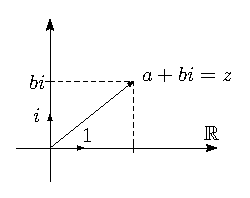
\includegraphics[width=0.25\textwidth]{AL1S1_1.eps}
	\caption{Визуализация комплексного числа.}
	\label{1_1}
\end{figure}
Мы натягиваем на $\MR$ и на новый символ $i$ плоскость $\Rightarrow$ каждый вектор записывается в виде:
$$
	z = a + bi, \, a,b \in \MR
$$ 
где $a$ - \uwave{действительная часть}, $b$ - \uwave{мнимая часть}:
$$
	\RE{(z)} = a \in \MR,\, \IM{(z)} = b \in \MR, \, z \in \MC
$$
геометрически действительная часть - абсцисса, мнимая часть - ордината. Формально, комплексное число это пара чисел $(a,b), \, a,b \in \MR$.  \uwave{Переменожение комплексных чисел} равно:
$$
	(a + bi)(c + di) = ac - bd + (ad + bc)i
$$
\uwave{Модуль комплексного числа} это геометрическое расстояние до нуля:
$$
	|z| = \sqrt{a^2 + b^2}
$$
\begin{problem}(\textbf{К20.1 а)}) 
	$$
		(2 + i)(3 -i) + (2+ 3i)(3 + 4i)
	$$
\end{problem}
\begin{proof}
	$$
		(2 + i)(3 -i) + (2+ 3i)(3 + 4i) = 6 + 1 + (-2 + 3)i + 6 -12 +(8 + 9)i = 1 + 18i
	$$
\end{proof}

\begin{problem}(\textbf{К20.1 и)}) 
	$$
		(2 + i)^3 + (2 - i)^3 
	$$
\end{problem}
\begin{proof}
	$$
		(2 + i)^3 + (2 - i)^3 = 8 + 3{\cdot}4{\cdot}i + 3{\cdot}2{\cdot}i^2 + i^3 + 8 - 3{\cdot}4{\cdot}i + 3{\cdot}2{\cdot}i^2 - i^3 = 16 -12 = 4
	$$
\end{proof}

\newpage
\begin{problem}(\textbf{К20.2}) 
	Вычислить:
	\begin{enumerate}[label=\arabic*)]
		\item $i^{77} $;
		\item $i^{98} $; 
		\item $i^{-57} $;
		\item $i^n, \, n \in \MZ $;
	\end{enumerate}
\end{problem}
\begin{proof}\hfill
	\begin{enumerate}[label=\arabic*)]
		\item $ i^{77} = i^{76}{\cdot}i = i^{19{\cdot}4}{\cdot}i = 1{\cdot}i = i$;
		\item $ i^{98} = i^{96}{\cdot}i^{2} = 1{\cdot}(-1) = -1, \, 96 = 4{\cdot}24$;
		\item $i^{-57} = i^{-1}{\cdot}i^{-14{\cdot}4} = \dfrac{1}{i} = \dfrac{i}{i^2} = -i $
		\begin{figure}[H]
			\centering
			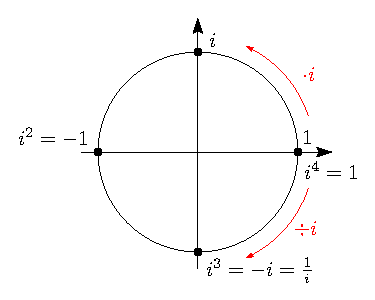
\includegraphics[width=0.35\textwidth]{AL1S1_2.eps}
			\caption{Визуализация умножения и деления на комплексное число.}
			\label{1_2}
		\end{figure}
		\item Рассмотрим $4$ случая:
		$$
			i^n = 
			\begin{cases}
				1, & n = 4k \\
				i, & n = 4k + 1 \\ 
				-1, & n = 4k + 2 \\
				-i,	& n = 4k + 3 
			\end{cases}, \, k \in \MZ
		$$
		поскольку $n = 4k + r, \, r \in \{0,1,2,3\} \Rightarrow i^n = (i^4)^k{\cdot}i^r = i^r$;
	\end{enumerate}
\end{proof}

\begin{problem}(\textbf{К20.11} а)) 
	Решить уравнение:
	$$
		z^2 = i
	$$
\end{problem}
\begin{proof}
	Пусть $z = a + bi \in \MC$, тогда:
	$$
		 z^2 = a^2  - b^2 + 2abi = i\Rightarrow 
		\begin{cases}
			2ab = 1 \\
			a^2 -b^2 = 0
		\end{cases} \Rightarrow 		
		\begin{cases}
			a = \pm b\\
			2ab = 1
		\end{cases} \Rightarrow 
		\begin{cases}
			a = \pm \dfrac{1}{\sqrt{2}}\\[10pt]
			b = \pm \dfrac{1}{\sqrt{2}}
		\end{cases} \Rightarrow z = \pm \left(\dfrac{1}{\sqrt{2}} + i \dfrac{1}{\sqrt{2}}\right)
	$$
\end{proof}

\uwave{Сопряженным к комплексному числу} $z = a + bi$ называется число:
$$
	\overline{z} = a - bi
$$
\begin{figure}[H]
	\centering
	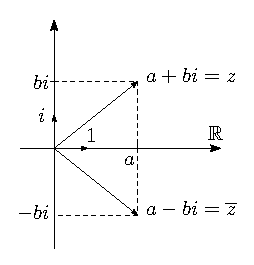
\includegraphics[width=0.25\textwidth]{AL1S1_3.eps}
	\caption{Сопряженное комплексное число $\overline{z}$ к $z$.}
	\label{1_3}
\end{figure}
геометрически это число симметричное числу $z$ относительно $\MR$ (действительной прямой). Произведение сопряженных равно:
$$
	z{\cdot}\overline{z} = a^2 +b^2 + (ab - ab)i = a^2 + b^2 = |z|^2
$$
\textbf{Свойства сопряжения}:
\begin{enumerate}[label=\arabic*)]
	\item $\overline{z + w} = \overline{z} + \overline{w}$;
	\item $\overline{z{\cdot}w} = \overline{z}{\cdot}\overline{w}$;
	\item $\overline{z^n} = \overline{z}^n, \, n \in \MN$;
\end{enumerate}
\begin{proof}\hfill
	\begin{enumerate}[label=\arabic*)]
		\item Пусть $z = a + bi, \, w = c + di$, тогда:
		$$
			\overline{z + w} = \overline{(a +c) + (b+ d)i} = (a+ c) - (b+d)i = a -bi + c - di = \overline{z} + \overline{w}
		$$	
		\item Пусть $z = a + bi, \, w = c + di$, тогда:
		$$
			\overline{z{\cdot}w} = \overline{ac - bd + (ad +bc)i} = ac -bd - (ad + bc)i = (a - bi)(c -di) = \overline{z}{\cdot}\overline{w}
		$$
		\item Пусть $z = a + bi$, тогда по индукции:
		$$
			n = 1 \Rightarrow \overline{z^1} = \overline{z}
		$$
		Пусть верно для $n$, рассмотрим для $n+1$:
		$$
			\overline{z^{n+1}} = \overline{z^n{\cdot}z} = \overline{z^n}{\cdot}\overline{z} = \overline{z}^n{\cdot}\overline{z} = \overline{z}^{n+1}
		$$
	\end{enumerate}
\end{proof}

\uwave{Деление комплексных чисел} имеет следующий вид:
$$
	\dfrac{1}{a + bi} = \dfrac{a -bi}{(a+ bi)(a-bi)} = \dfrac{a - bi}{a^2 + b^2} = \dfrac{a}{a^2+b^2} - \dfrac{b}{a^2+ b^2}i = \dfrac{a}{|z|^2} - \dfrac{b}{|z|^2}i = \dfrac{1}{|z|^2}(a- bi) = \dfrac{\overline{z}}{|z|^2}
$$

\begin{problem}(\textbf{К20.1 л)}) 
	$$
		\dfrac{(1 + i)^5}{(1-i)^3}
	$$
\end{problem}
\begin{proof}
	$$
		\dfrac{(1 + i)^5}{(1-i)^3} = \dfrac{(1+i)^5{\cdot}(1+i)^3}{|(1+i)|^3} = \dfrac{(1+i)^8}{8} = \dfrac{((1+i)^2)^4}{8} = \dfrac{(1 +2i -1)^4}{8} = \dfrac{2^4 {\cdot}i^4}{8} = 2
	$$	
\end{proof}
Отметим некоторые свойства комплексных чисел:
\begin{enumerate}[label=\arabic*)]
	\item $z = \overline{z} \Leftrightarrow z \in \MR$;
	\item $z = - \overline{z} \Leftrightarrow z \in i\MR$;
	\item $z = \dfrac{1}{\overline{z}} \Leftrightarrow |z|^2 = 1 \Leftrightarrow |z| = 1$;
\end{enumerate}
\begin{proof}\hfill
	\begin{enumerate}[label=\arabic*)]
		\item $z = \overline{z} \Leftrightarrow a + bi = a- bi \Leftrightarrow b = 0 \Leftrightarrow z = a \in \MR$;
		\item $z = -\overline{z} \Leftrightarrow a + bi = -a +bi \Leftrightarrow a = 0 \Leftrightarrow z = ib \in i\MR$;
		\item $z = \dfrac{1}{\overline{z}} \Leftrightarrow z{\cdot}\overline{z} = 1 \Leftrightarrow |z| = 1$;
	\end{enumerate}
\end{proof}
\begin{rem}
	Числа, которые обратны своим сопряженным это в точности числа, которые лежат на еденичной окружности.
\end{rem}

\begin{problem}(\textbf{К24.3}) 
	Какой геометрический смысл у $|z_1 - z_2|$, где $z_1, z_2 \in \MC$.
\end{problem}
\begin{proof}
	Как и на прямой, смысл разности - расстояние между $z_1,z_2$.
	\begin{figure}[H]
		\centering
		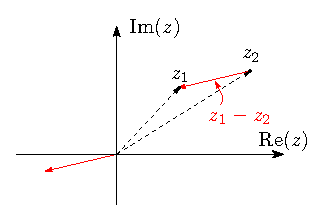
\includegraphics[width=0.4\textwidth]{AL1S1_4.eps}
		\caption{Геометрический смысл $|z_1 - z_2|$.}
		\label{1_4}
	\end{figure}
	Геометрический смысл модуля разности - расстояние до нуля: производится параллельный сдвиг (от этого расстояние не меняется) и получается расстояние от $z_1$ до $z_2$.
\end{proof}
\newpage
\begin{problem}(\textbf{К24.6}) 
	Изобразить на плоскости множество точек:\hfill\\
	а) $|z| = 1$;\\
	в) $|z| \leq 2$;\\
	г) $|z - 1 - i| < 1$;\\
	к) $-1 < \RE{(iz)} < 0$;
\end{problem}
\begin{proof}\hfill\\
	а) единичная окружность.
	\begin{figure}[H]
		\centering
		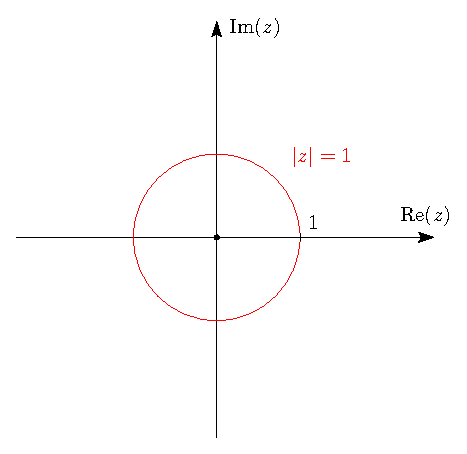
\includegraphics[width=0.4\textwidth]{AL1S1_5.eps}
		\caption{Пункт а).}
		\label{1_5}
	\end{figure}
	в) круг с центром в $0$ радиуса $2$.
	\begin{figure}[H]
		\centering
		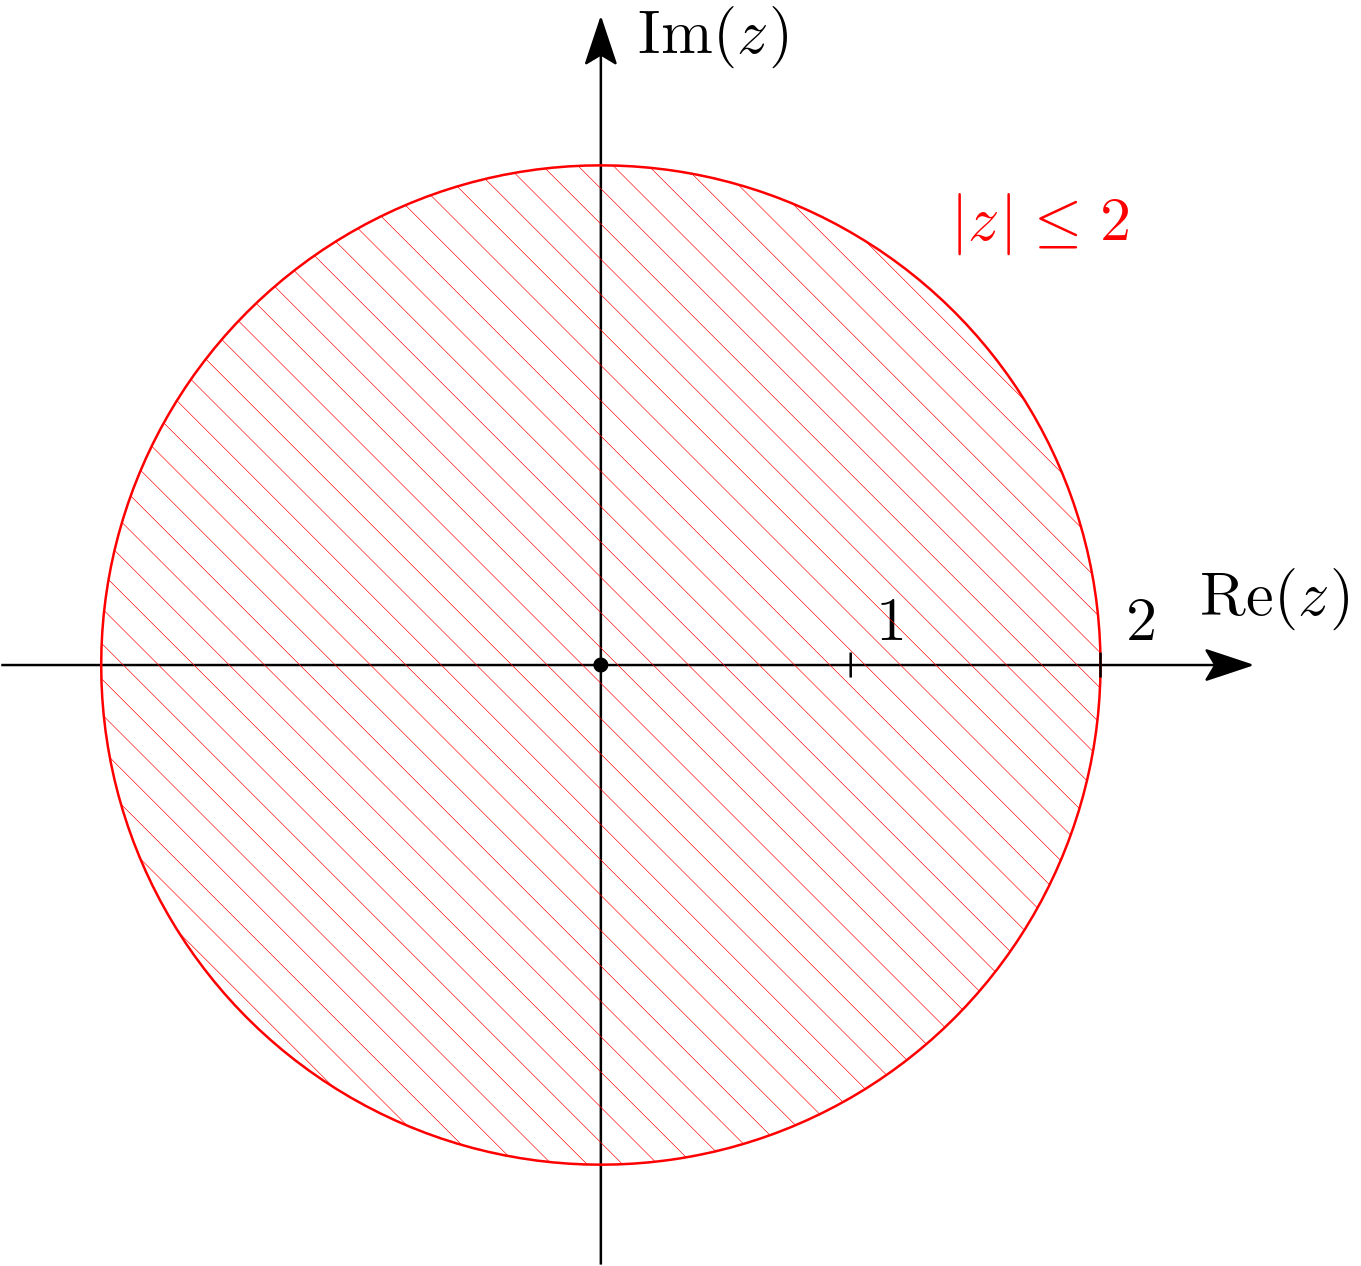
\includegraphics[width=0.4\textwidth]{AL1S1_6.png}
		\caption{Пункт в).}
		\label{1_6}
	\end{figure}
	\newpage
	г) открытый круг радиусом $1$ и центром в точке $1 + i$.
	\begin{figure}[H]
		\centering
		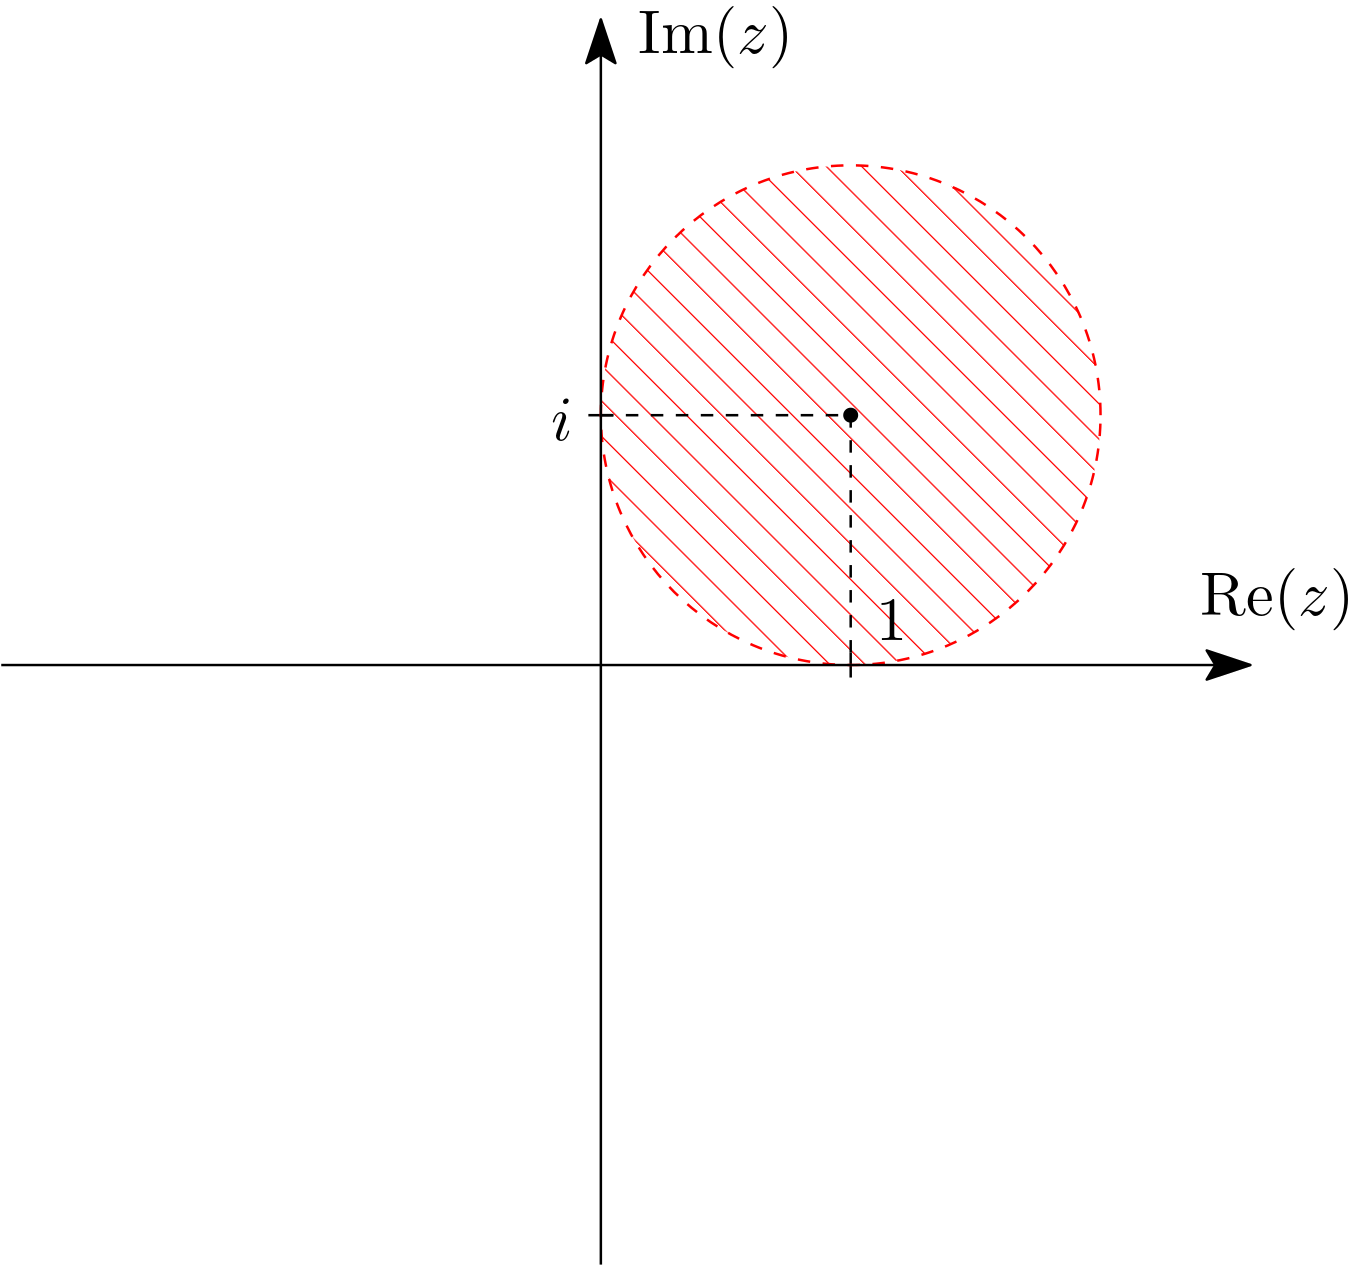
\includegraphics[width=0.4\textwidth]{AL1S1_7.png}
		\caption{Пункт г).}
		\label{1_7}
	\end{figure}
	к) пусть $z =a + bi \Rightarrow iz  = -b + ai, \, \RE{(iz)} = -b \Rightarrow$ получаем полосу $0 < b < 1$.
	\begin{figure}[H]
		\centering
		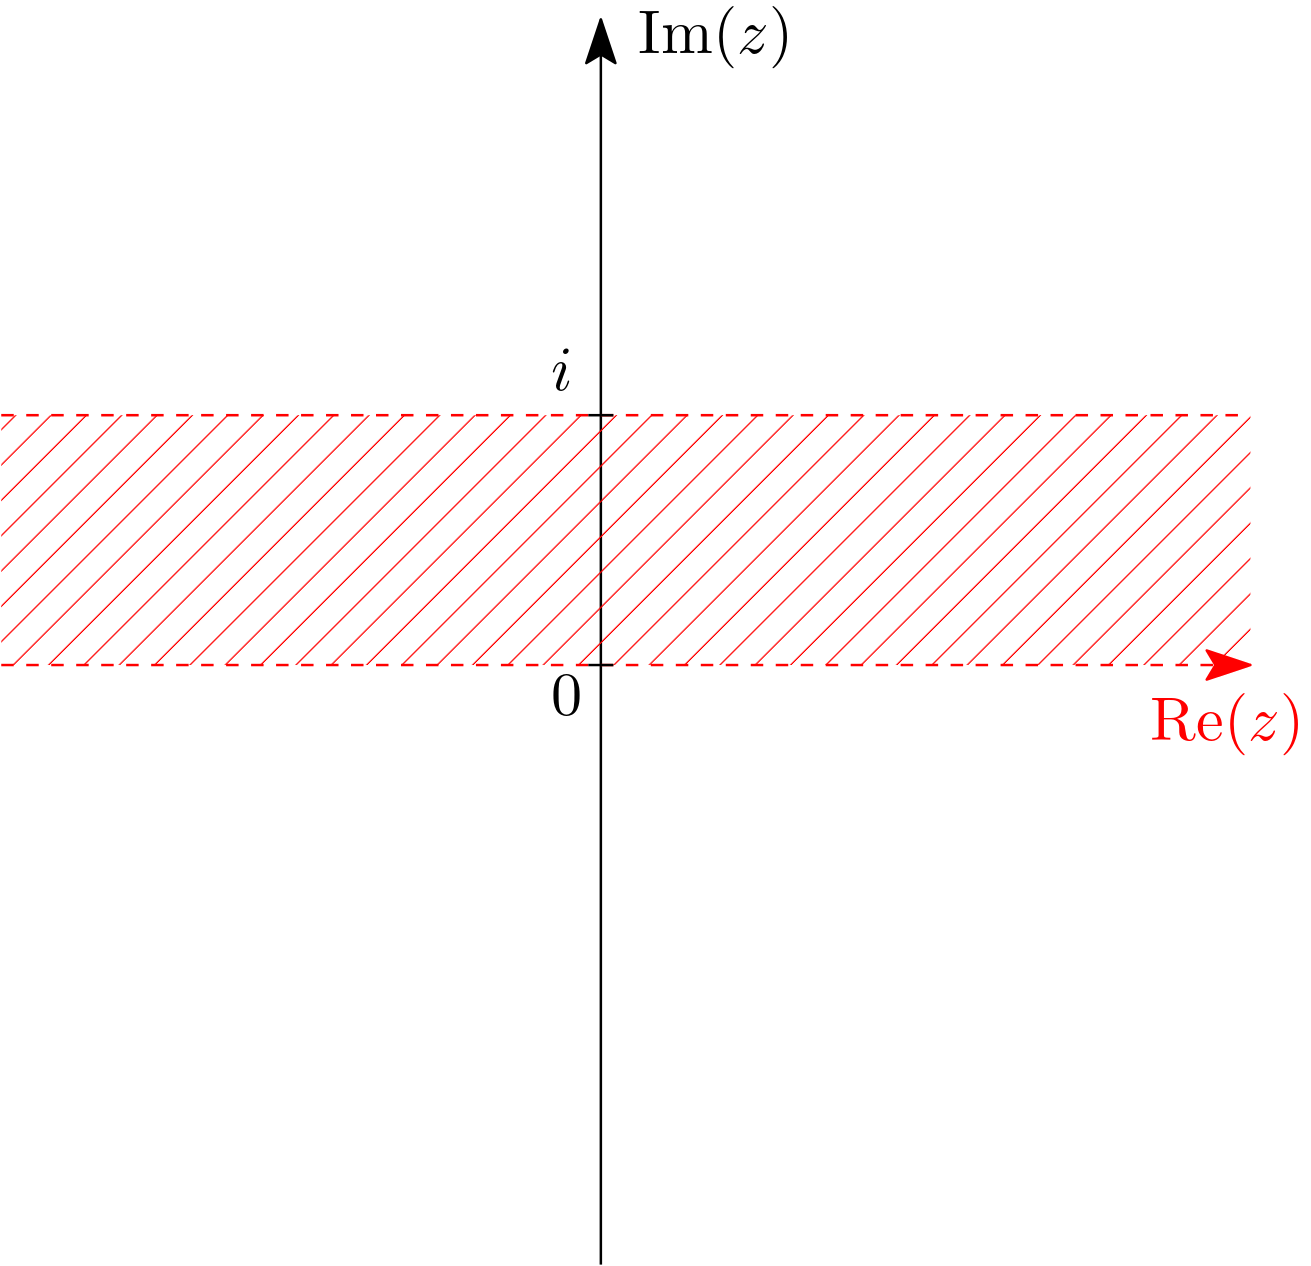
\includegraphics[width=0.4\textwidth]{AL1S1_8.png}
		\caption{Пункт к).}
		\label{1_8}
	\end{figure}
\end{proof}

\textbf{ДЗ}: $20.1$ бгем, $20.3$ б, $20.5$ a, $20.7$ б, $20.8$ a, $24.2$ б, $24.6$ дмн.

\end{document}